%\ctparttext{\color{black}\begin{center}
%		Esta es una descripción de la parte de informática.
%\end{center}}

%\part{Parte de informática}
\chapter{Análisis y diseño}

\section{Objetivos y análisis de requisitos}

Los objetivos que se persiguen al realizar este proyecto son realizar un estudio de distintos modelos de epidemiología, comprendiendo cómo afectan sus parámetros y condiciones iniciales a la evolución en el tiempo de estos modelos, desde un punto de vista tanto teórico como práctico, apoyándonos en distintas gráficas interactivas para ilustrar dichos comportamientos. Asimismo, se va a analizar la bondad de ajustes de parámetros de algunos de los modelos presentados aplicados a datos reales, comprobando cuáles proporcionan mejores resultados en cada caso. Con el fin de satisfacer todos estos objetivos, se ha extraído la siguiente lista de requisitos:

\begin{itemize}
\item \textbf{Requisitos funcionales}
	\begin{itemize}
	\item \textbf{RF1} Se debe poder modificar los parámetros de las gráficas de los distintos modelos.
	\item \textbf{RF2} El usuario debe poder elegir con qué modelo quiere trabajar.
	\item \textbf{RF3} El sistema debe permitir descargar las imágenes de las gráficas obtenidas.
	\item \textbf{RF4} El sistema debe poder cargar y leer ficheros de datos.
	\item \textbf{RF5} Se debe visualizar el ajuste obtenido mediante gráficas.
	\item \textbf{RF6} Para cada ajuste realizado se obtendrá los valores estimados de los parámetros y los errores.
	\item \textbf{RF7} El sistema debe ser capaz de seleccionar qué modelo se ajusta mejor a los datos. 
	\end{itemize}
\item \textbf{Requisitos no funcionales}
	\begin{itemize}
	\item \textbf{RNF1} No se podrán ajustar datos de más de un fichero a la vez.
	\item \textbf{RNF2} Las gráficas deben ser en tiempo real
	\item \textbf{RNF3} Se mostrará información de ayuda, en caso de ser necesaria.
	\item \textbf{RNF4} Se debe poder usar desde el navegador.
	\end{itemize}
\item \textbf{Requisitos de información}
	\begin{itemize}
	\item \textbf{RI1} Los ficheros de datos con los que se va a trabajar deben ser formato csv con una estructura específica, dependiente de cada modelo.
	\end{itemize}
\end{itemize}

\section{Desarrollo del proyecto}

Actualmente hay diversas metodologías de desarrollo del software. Cada uno de estos modelos consta de una serie de etapas en las que se ha dividido el desarrollo. Para este proyecto, se ha optado por el modelo en espiral. En este modelo el software se desarrolla de forma incremental, es decir, se van añadiendo funcionalidades y mejoras al software según se van evaluando las que ya tiene. Cada bucle o iteración representa un conjunto de actividades. Estas actividades no están fijadas a ninguna prioridad, sino que las siguientes se eligen en función del análisis de riesgo, comenzando por el bucle interior. \eqref{modelo_espiral}

\begin{figure}
\begin{center}
\caption{Modelo en espiral.}
\label{modelo_espiral}
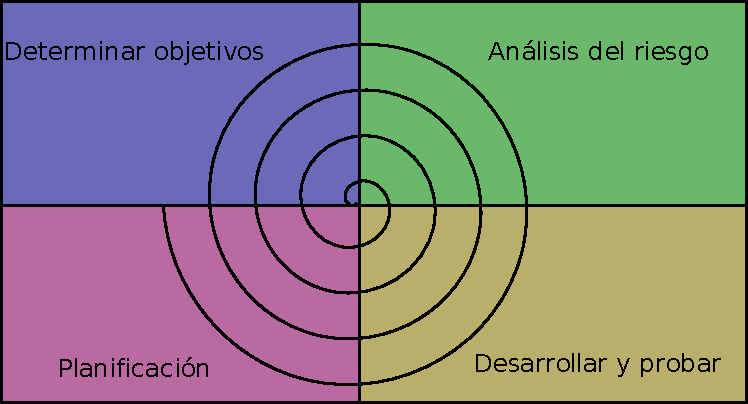
\includegraphics[scale=1]{modelo_espiral}
\end{center}
\end{figure}

\section{Gestión de recursos}

Los proyectos que se pueden realizar dependen en gran medida de los recursos que se pueden destinar a ellos. Se requiere de unos elementos mínimos que son indispensables para poder llevarlo a cabo. Por ello, es muy importante contar con los recursos necesarios y gestionarlos de manera adecuada.

\subsection{Recursos humanos}

El proyecto consta de un equipo de 3 personas para llevarlo a cabo:

\begin{itemize}
\item Ana Buendía Ruiz-Azuaga, se encarga de:
	\begin{itemize}
	\item Planificación y análisis del proyecto.
	\item Búsqueda de bibliografía.
	\item Diseño e implementación del proyecto.
	\item Pruebas para el correcto funcionamiento del proyecto.
	\item Redacción de la documentación del proyecto.
	\end{itemize}
\item Tutores: Manuel Pegalajar Cuéllar y Teresa E. Pérez, encargados de:
	\begin{itemize}
	\item Proporcionar bibliografía.
	\item Guiar para la redacción de la memoria y documentación.
	\item Supervisar el desarrollo del proyecto.
	\end{itemize}
\end{itemize}

\subsection{Recursos hardware}

Todo el proyecto se va a desarrollar en un ordenador portátil con todo el software y dependencias necesarias. Las especificaciones del portátil son:

\begin{itemize}
\item \textbf{Modelo}: Acer Aspire E-5 574G.
\item \textbf{CPU}: Intel Core i5-6200U.
\item \textbf{RAM} 8GB RAM DDR3.
\item \textbf{Disco duro}: 1TB.
\item \textbf{Precio}: 600€.
\end{itemize}

\subsection{Recursos software}

El proyecto se ha llevado a cabo usando como sistema operativo Ubuntu 20.04 LTS, y se ha usado como lenguaje principal Python.

El software necesario para el proyecto es el siguiente:

\begin{itemize}
\item \textbf{Flask}. Flask es un microframework web en python. Proporciona funcionalidad básica para, de forma sencilla, crear una aplicación web. Una posible alternativa habría sido Django, pero finalmente se ha optado por Flask debido a su simplicidad, legibilidad y que en este proyecto no se requieren muchas de las funcionalidades que Django ofrece integradas. 
\item \textbf{Dash}. Dash es un framework opensource basado en plotly.js y react.js que permite crear fácilmente aplicaciones basadas en datos. En este proyecto, se ha usado principalmente por su capacidad de crear gráficas interactivas en tiempo real. 
\item \textbf{VSCode}. Se ha usado VSCode como editor de texto, ya que proporciona una gran cantidad de plugins para cualquier lenguaje, así como integración con git.
\item \textbf{Draw.io}. Para la realización de diagramas de distintas clases, se ha usado el software de dibujo gratuito Draw.io.
\item \textbf{Docker}. Con el fin de simplificar el lanzamiento y ejecución de la aplicación web desarrollada se ha usado docker para virtualizar el entorno y evitar la necesidad de instalar en cualquier máquina el software necesario para ejecutarla.
\item \textbf{Git}. Se ha empleado Git como controlador de versiones, integrado con Github.
\item \textbf{Texmaker}. Para redactar la memoria, se ha usado el editor de LaTeX Texmaker.
\end{itemize}

Todo el software utilizado ha sido gratuito, por lo que no ha tenido coste alguno.

\subsection{Estimación del coste}

A partir de los recursos previamente listados, se va a realizar una aproximación del coste de la consecución del proyecto, considerando que la duración del mismo es de 9 meses.

Para los recursos humanos, dado que se considera que la alumna ha trabajado aproximadamente 450 horas de acuerdo a los créditos correspondientes asignados al TFG, y el gasto aproximado es 15€/h en calidad de alumna de prácticas, se tiene que el coste es de 6750€.

A los tutores, dada su formación profesional se les supone un coste estimado de 50€/h, y aproximando que se dedican 3 horas semanales para la tutorización del proyecto, se tiene que el coste total tras los 9 meses es de 5400€ por tutor.

Dado que el portátil empleado tiene una vida útil estimada de 5 años, le corresponde un coste de 120€ durante la realización del proyecto.

Finalmente, dado que todo el software empleado es gratuito, el coste aproximado del proyecto se puede ver en \eqref{tabla_pres}.

\begin{table}[!h]
\caption{Desglose de presupuesto del proyecto.}
\begin{center}
\begin{tabular}{|c c|} 
 \hline
 \textbf{Recursos humanos} & \textbf{Coste (€)} \\ 
 \hline\hline
 Alumna & 6750 \\
 \hline
 Tutor 1 & 5400 \\
 \hline 
 Tutor 2 & 5400 \\
 \textbf{Suma} & \textbf{17550} \\
 \hline
 \textbf{Recursos hardware} & \textbf{Coste (€)} \\ 
 \hline\hline
 Ordenador portátil & 120 \\
 \hline
 \textbf{Suma} & \textbf{120} \\
 \hline 
 \textbf{Recursos software} & \textbf{Coste (€)} \\
 \hline
  Flask & 0 \\
  \hline
  Dash & 0 \\
  \hline 
  VSCode & 0 \\
  \hline
  TexMaker & 0 \\
  \hline 
  \textbf{Suma} & \textbf{0} \\ 
 \hline\hline
 \textbf{Suma total} & \textbf{17670} \\
 \hline\hline
 \textbf{Gastos indirectos (18\%)} & \textbf{3180.6} \\ 
 \hline\hline
 \textbf{Total} & \textbf{20850.6)} \\ 
 \hline\hline
 \textbf{IVA (21\%)} & \textbf{4378.626} \\ 
 \hline\hline
 \textbf{Coste final} & \textbf{25229.226} \\ 
 \hline\hline

 \hline
\end{tabular}
\label{tabla_pres}
\end{center}
\end{table}

\section{Planificación temporal}



\section{Diagrama conceptual}

Para el modelado conceptual de la aplicación web, se ha optado por utilizar OOWS (Object-Oriented approach for Web Solutions modelling), que usa modelado de objetos UML y modelos de navegación y presentación usando UML. Así, se expresan las características navegacionales de la aplicación web a la vez que se integra con las restantes vistas del esquema conceptual mediante una notación UML adaptada.

En \eqref{diag: modelo_concep}, se muestra el diagrama conceptual, construido mediante una estrategia top-down:

\begin{figure}[!h]
\begin{center}
\caption{Modelo conceptual de la aplicación web.}
\label{diag: modelo_concep}
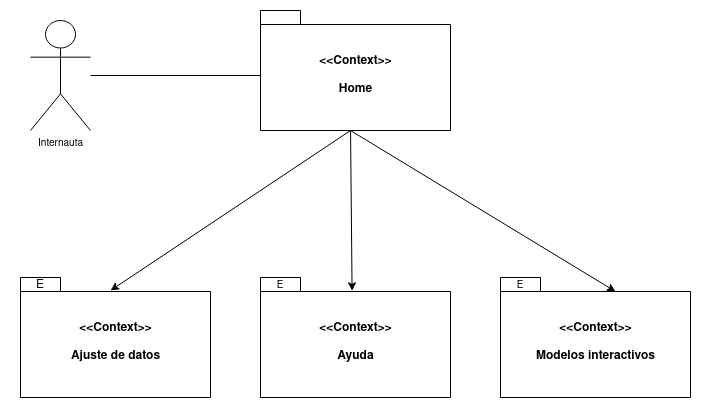
\includegraphics[scale=0.5]{modelo_conceptual-vista-paquetes.drawio}
\end{center}
\end{figure}

En \eqref{diag: modelo_concep_home} se muestra el detalle del contexto de \verb|Home|, en \eqref{diag: modelo_concep_modelos} se ve el detalle de \verb|Modelos Interactivos|, así como en \eqref{diag: modelo_concep_ayuda} el de \verb|Ayuda| y en \eqref{diag: modelo_concep_ajuste} el de \verb|Ajuste de datos|.

\begin{figure}[!h]
\begin{center}
\caption{Modelo conceptual del contexto de Inicio.}
\label{diag: modelo_concep_home}
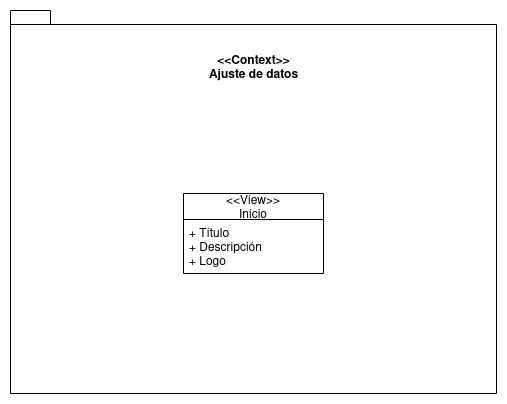
\includegraphics[scale=0.5]{modelo_conceptual-home.drawio}
\end{center}
\end{figure}

\begin{figure}[!h]
\begin{center}
\caption{Modelo conceptual del contexto de Modelos Interactivos.}
\label{diag: modelo_concep_modelos}
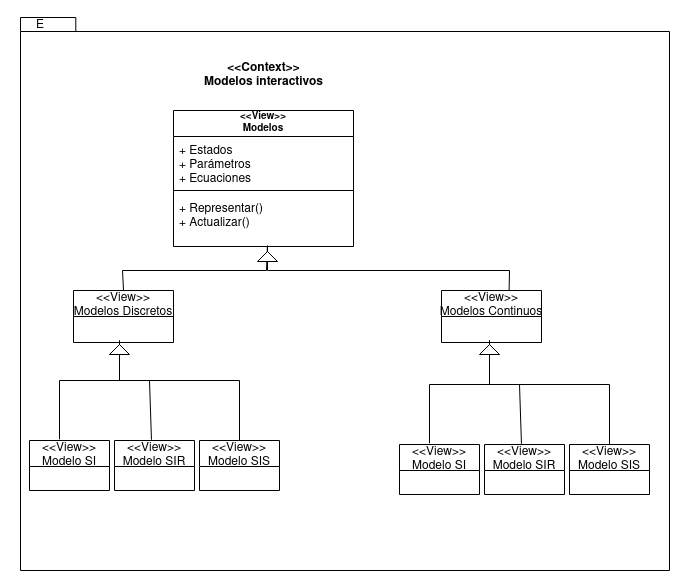
\includegraphics[scale=0.5]{modelo_conceptual-Modelos.drawio}
\end{center}
\end{figure}

\begin{figure}[!h]
\begin{center}
\caption{Modelo conceptual del contexto de Ayuda.}
\label{diag: modelo_concep_ayuda}
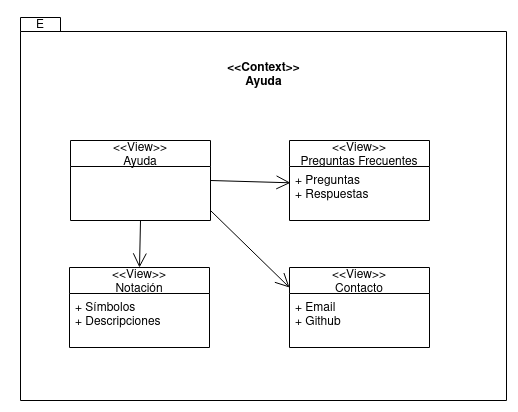
\includegraphics[scale=0.5]{modelo_conceptual-Ayuda.drawio}
\end{center}
\end{figure}

\begin{figure}[!h]
\begin{center}
\caption{Modelo conceptual del contexto de Ajuste de Datos.}
\label{diag: modelo_concep_ajuste}
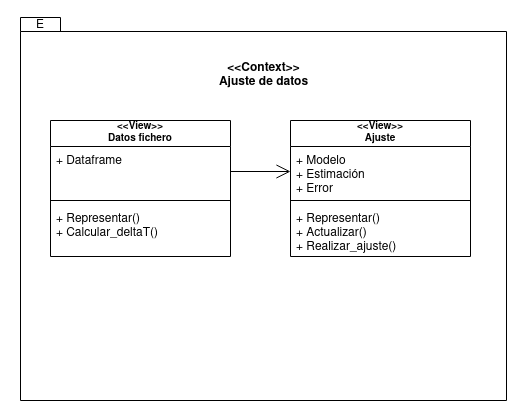
\includegraphics[scale=0.5]{modelo_conceptual-Ajuste.drawio}
\end{center}
\end{figure}







\section{Pruebas unitarias}



\section{Casos de uso}












